\documentclass[aspectratio=169]{beamer}
\usepackage{basileabeam}
\addbibresource{presentation.bib}
% Notes:
%\pgfpagesuselayout{2 on 1}[a4paper,border shrink=5mm]
%\setbeamertemplate{note page}[plain]
%\setbeameroption{show notes on second screen=bottom}

\title              {Application of Graph Learning to inverse problems}

\author     		{Cédric Mendelin}
\email				{cedric.mendelin@stud.unibas.ch}
\institute          {Department of Mathematics and Computer Science, University of Basel}

\date               {Date}

\ulogo        		{Template/header}
\ulistelement    	{Template/listelement}

\graphicspath{{Figures/}}

% Options:
%\totalNoSlidesDisabled % To turn off the total number of slides in the footer. Comment this if you want the total number of slides in the footer

%\headerSectionsDisabled % Comment this if you want a fancy header containing your sections.


\begin{document}

\begin{frame}[t,plain]
    \titlepage
\end{frame}

\begin{frame}[t]{Overview}
    \tableofcontents
\end{frame}

%% Presentation content

\section{Imaging methods}	% You can also have slides prior to the first section or work entirely without sections.


\begin{frame}[c]{Some Images}
\begin{columns}[c]
    \column{.55\textwidth}
            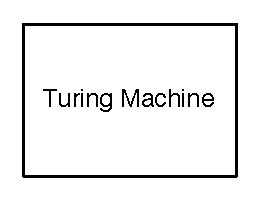
\includegraphics[width=0.8\textwidth]{block}
    \column{.45\textwidth}
            Turing machine \cite{diffusionMaps}
\end{columns}
\end{frame}


\begin{frame}[c]{Some Images}
    \begin{figure}
        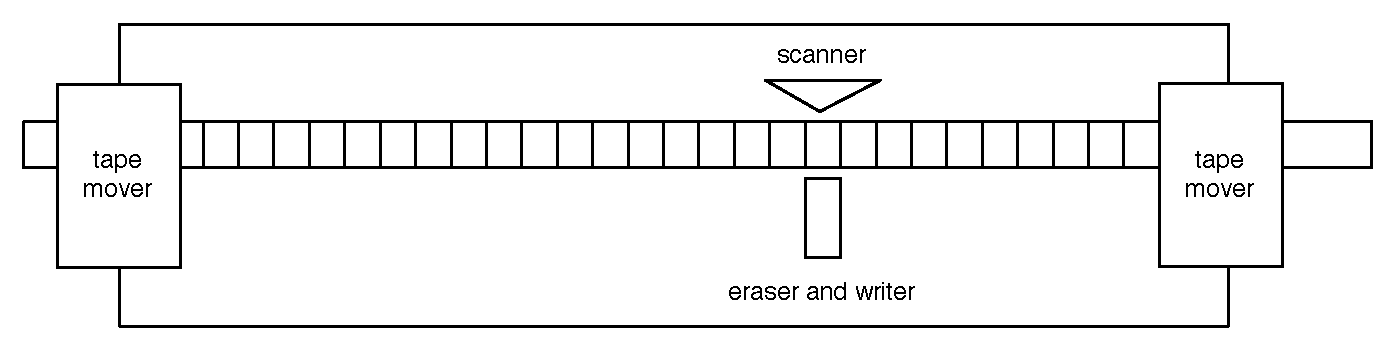
\includegraphics[width=0.8\textwidth]{turingmachine}
        \caption{A Turing Machine.}
    \end{figure}
\end{frame}


\begin{frame}[c]{Some Equations}
Now we introduce an equation.
\begin{theorem}
A Turing Machine is a 7-Tuple:
\begin{equation}
    M = \langle Q, \Gamma, b, \Sigma, \delta, q_0, F \rangle
\end{equation}
\end{theorem}
A Turing Machine is a 7-Tuple even if defined in the text, as in $M = \langle Q, \Gamma, b, \Sigma, \delta, q_0, F \rangle$.
\end{frame}


\section{Graph Denoising}

\begin{frame}{Graph construction}
    Let $\Omega$ be a dataset $\Omega \subset \mathbb{R}^M$, a graph can be constructed like:
    \begin{itemize}
        \item $V$: each node associated with $x \in \Omega$
        \item $E$: Calculate adjacency matrix with similarity measure $d$ and some threshold $\tau$
     \end{itemize}

    \begin{columns}
        \column{.5\textwidth}
            \begin{definition}
                \begin{equation}
                    \label{eq:graphConstruction}
                    A_{ij} =    
                    \begin{cases}
                        1  & \text{if } d(x_i, x_j) < \tau\\
                        0, & \text{otherwise}
                    \end{cases}
                \end{equation}
            \end{definition}
        \column{.5\textwidth}
    \end{columns}
\end{frame}

\begin{frame}{Graph construction}
    Let $\Omega$ be a dataset $\Omega \subset \mathbb{R}^M$, but only observation 
    of $y = x + \eta$ (with $\eta$ drawn from $\mathcal{N} \sim (0, \sigma^2)$), 
    a graph can be constructed like:
    \begin{itemize}
        \item $V$: each node associated with $y \in \Omega$
        \item $E$: Calculate adjacency matrix with similarity measure $d$ and some threshold $\tau$
     \end{itemize}

    \begin{columns}
        \column{.5\textwidth}
            \begin{definition}
                \begin{equation}
                    \label{eq:graphConstruction}
                    A_{ij} =    
                    \begin{cases}
                        1  & \text{if } d(x_i, x_j) < \tau\\
                        0, & \text{otherwise}
                    \end{cases}
                \end{equation}
            \end{definition}
        \column{.5\textwidth}
            \begin{definition}
                \begin{equation}
                    \label{eq:graphConstructionNoise}
                    A_{0_{ij}} =    
                    \begin{cases}
                        1  & \text{if } d(y_i, y_j) < \tau\\
                        0, & \text{otherwise}
                    \end{cases}
                \end{equation}
                
            \end{definition}
    \end{columns}
\end{frame}

\begin{frame}[c]{Noisy graph}

    \begin{theorem}
        For every noisy graph $G_0 = \langle V, E_0 \rangle$, 
        there exists a noiseless graph $G = \langle V, E \rangle$.
        Both graphs consists of the same set of vertices $V$ but different edges.
        $E_0$  is defined as follows:
        $$E_0 = E \setminus  E^{-}_0 \cup  E^{+}_0,$$
        where $E^{-}_0 \subseteq E$ and $E^{-}_0 \subseteq U$ with $U$ the set of all possible edges and $E^{+}_0 \cap E = \emptyset$
    \end{theorem}

\end{frame}

\begin{frame}[c]{Graph Denoising}
    \textit{Graph denoising} is the task, to estimate a denoised graph $\tilde{G}$  
    from a given noisy graph $G_O$, with underlying original graph $G$:

    \begin{definition}
        $$GD: G_0 \mapsto \tilde{G} \approx G,$$
    \end{definition}
    where $G_0$, $\tilde{G}$, $G$ denotes noisy, estimated denoised and original graph respectively.
    
    \begin{definition}
        $$GD: A_0 \mapsto \tilde{A} \approx A,$$
    \end{definition}
    where $A_0$, $\tilde{A}$, $A$ denotes adjacency matrix from $G_0$, $\tilde{G}$ and $G$ respectively.

\end{frame}

\section{Conclusion}


\begin{frame}[t]{Items and Numbers}
\begin{columns}
    \column{.5\textwidth}
            \begin{itemize}
            \item one
            \item two
            \item three
            \end{itemize}
    \column{.5\textwidth}
            \begin{enumerate}
            \item first
            \item second
            \item third
            \end{enumerate}
\end{columns}
\end{frame}


\begin{frame}[t,plain]
\lastpage{{\usebeamerfont{title} Questions?}\\[5ex]}
\end{frame}

\backupbegin

%\begin{frame}{References}
%    \printbibliography
%\end{frame}

\backupend

\end{document}

